\documentclass[tikz]{standalone}
\usepackage{amsmath}
\usepackage{amssymb}
\usepackage{amsfonts}
\usepackage{tikz}
\usetikzlibrary{calc}
\usepackage{lmodern}

\thispagestyle{empty}
\begin{document}

 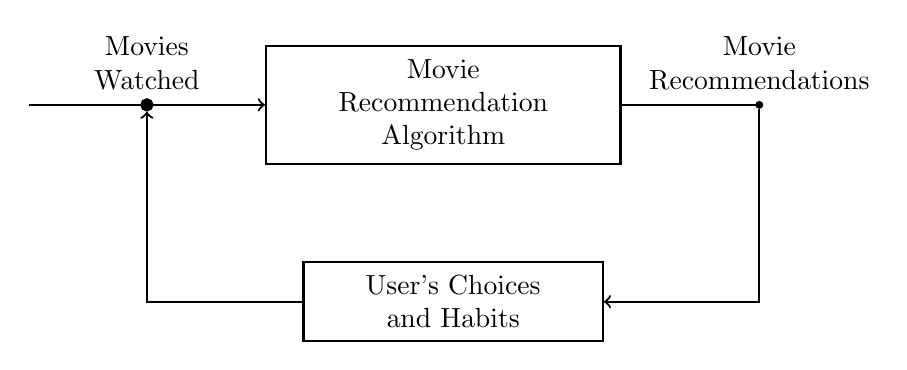
\begin{tikzpicture}[thick]
% Main algorithm block
\node[draw, rectangle, minimum width=4.5cm, minimum height=1.5cm, align=center] (block) at (0,0) {Movie\\Recommendation\\Algorithm};

% Input side
\coordinate (instart) at ($(block.west)+(-3,0)$);
\coordinate (inmid) at ($(block.west)+(-1.5,0)$);
\draw[->] (instart) -- (block.west);
\node[draw, circle, minimum size=4pt, inner sep=0pt, fill=black] (leftnode) at (inmid) {};
\node[align=center, above=2pt] at (leftnode) {Movies\\Watched};

% Output side
\coordinate (outend) at ($(block.east)+(1.75,0)$);
\coordinate (outmid) at ($(block.east)+(1.75,0)$);
\draw[-] (block.east) -- (outend);
\node[draw, circle, minimum size=2pt, inner sep=0pt, fill=black] (rightnode) at (outmid) {};
\node[align=center, above=2pt] at (rightnode) {Movie\\Recommendations};

% Feedback path with intermediate block
\coordinate (fbdown1) at ($(rightnode)+(0,-2.5)$);
\coordinate (fbdown2) at ($(leftnode)+(0,-2.5)$);

% User behavior filter block
\node[draw, rectangle, minimum width=3.8cm, minimum height=1cm, align=center] (filter) at ($(rightnode)!0.5!(leftnode)+(0,-2.5)$) {User's Choices\\and Habits};

% Connecting feedback arrows
\draw[->] (rightnode) -- (fbdown1) -- (filter.east);
\draw[->] (filter.west) -- (fbdown2) -- (leftnode);

\end{tikzpicture}

\end{document}
